\documentclass[a0paper]{tikzposter}

\usepackage{mathptmx}       % Mathematical PostScript fonts
\usepackage{multicol}

\hyphenpenalty=5000
\setlength{\columnsep}{2cm}

\definebackgroundstyle{samplebackgroundstyle}{
\draw[inner sep=0pt, line width=0pt, color=white]
(bottomleft) rectangle (topright);
}

\title{
    \begin{minipage}{\linewidth}\centering
        Cern Open Hardware Experience: Upgrading the Diamond Fast Archiver
        \vspace{1cm}
    \end{minipage}
}

\author{I.S.~Uzun and M.G.~Abbott}
\institute{Diamond Light Source, Oxfordshire, UK}

\usetheme{Envelope}
\usebackgroundstyle{samplebackgroundstyle}

\begin{document}

\maketitle

\begin{columns}
    \column{0.5}
    \block{Diamond FOFB Architecture}{
        \begin{center}
            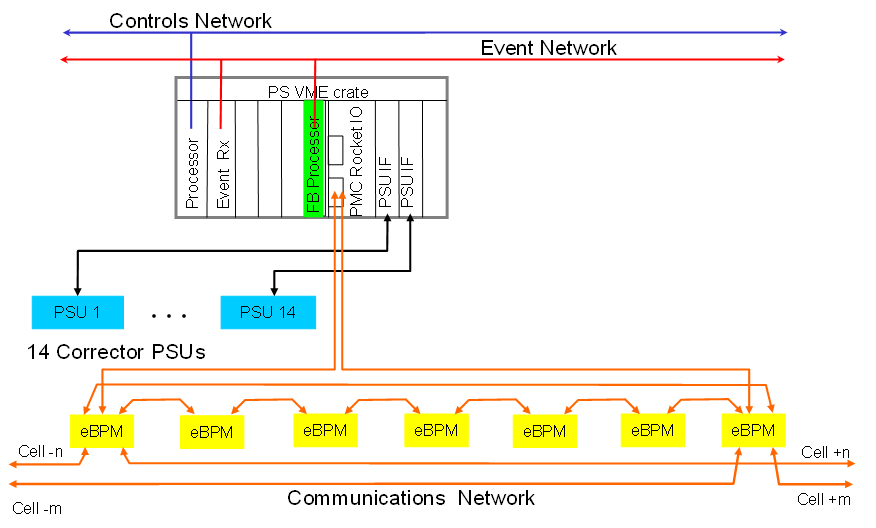
\includegraphics[scale=1.0]{img-poster/WEPGF089f1}
        \end{center}
    The system architecture for the FOFB for a single Storage Ring (SR) cell
    consists of 7 EBPMs, a PMC receiver, VME feedback processor and power supply
    controllers. Diamond SR consists of 24 cells.
    }

    \column{0.5}
    \block{Diamond Communication Network}{
        \begin{center}
            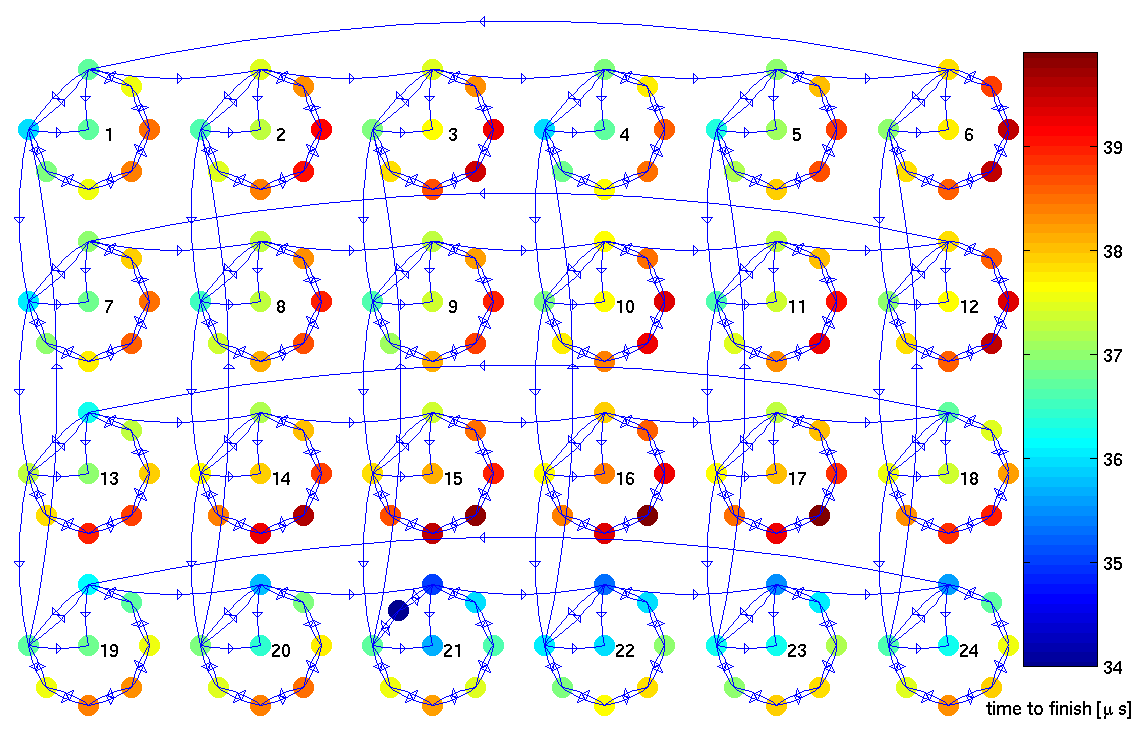
\includegraphics[scale=0.74]{img-poster/WEPGF089f3}
        \end{center}
        All Storage Ring EBPMs and PMC Receivers are connected to Communication
        Network in 2D Torus topology.
    }
\end{columns}


\begin{columns}
    \column{0.5}
    \block{The Fast Acquisition Archiver}{
        The FA archiver captures X,Y position data from a network of EBPMs and other sources at 10 kHz, maintains a rolling historical record and rebroadcasts the complete data stream to all interested parties. Other sources contributing to the network are a handful of X-ray BPMs and power pick-ups from the RF cavities.
        \begin{itemize}
            \item 512 X,Y position updates every 100 $\mu$s, sustained 40 MB/s.
            \item At Diamond we archive the last 14 days of orbit position.
            \item Any number of clients (limited by network connection to archive server) can read the archive and subscribe to the rebroadcast live data stream.
        \end{itemize}
    }

    \column{0.5}
    \block{Hardware Requirements for FA Archiver}{
        Implementation of FA archiver interface requires a PCIe form factor hardware platform with following on-board resources:
        \begin{itemize}
            \item Minimum 1-lane of PCIe bus interface. This could be either through dedicated IPs blocks on an FPGA device or a bridge chip external to the FPGA.
            \item At least 1 MGT on the FPGA for DCC implementation.
            \item On-board SFP connector(s) for physical connection to the communication network.
            \item Clocking resources required for PCIe, DMA data transfer and DCC FPGA logic.
        \end{itemize}
    }
\end{columns}


\begin{columns}
    \column{0.5}
    \block{FA Archiver in Context}{
        \begin{center}
            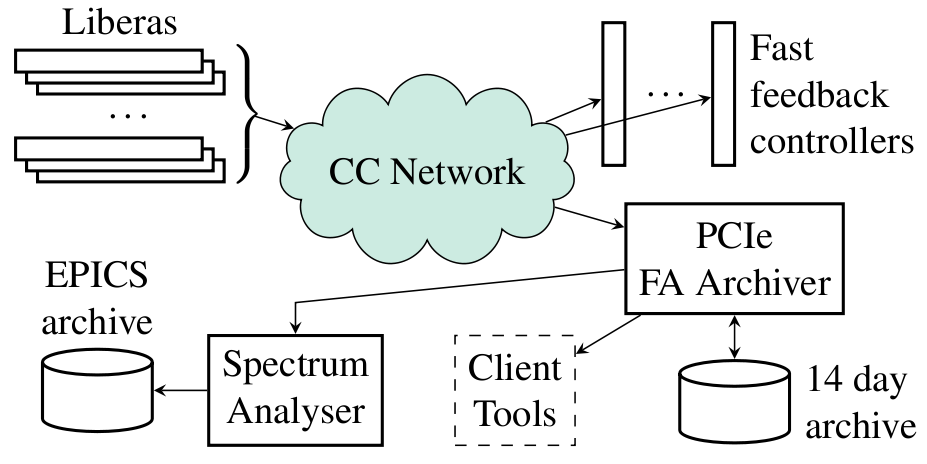
\includegraphics[scale=1.25]{img-poster/WEPGF089f4}
        \end{center}
        The FA archiver acts as a passive listener and makes the FA data freely available.
    }
    \column{0.5}
    \block{Existing Firmware Design on ML555 Card}{
    \begin{multicols}{2}
        \center
        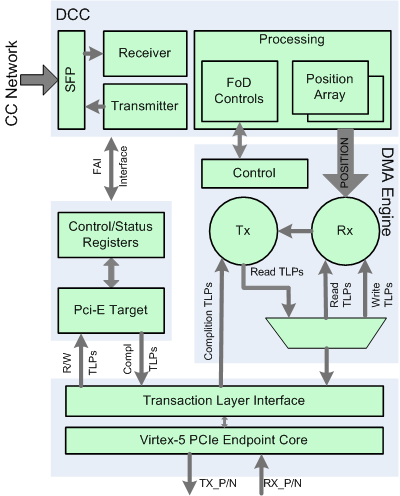
\includegraphics[scale=1]{img/WEPGF089f4}
        \begin{itemize}
            \setlength\itemsep{1em}
            \item Integrates the DCC into a bus master PCIe architecture on the ML555 FPGA board.
            \item Target logic is responsible for capturing  memory write and memory read PCIe Transaction Layer Packets (TLPs) for control and status register access.
            \item The DMA initiator logic generates memory write TLPs to transfer 4K byte frame data from the DCC core to the host system memory through PCIe endpoint.
        \end{itemize}
    \end{multicols}
     }
\end{columns}

\begin{columns}
    \column{0.3}
        \block{Motivation}{
            \begin{itemize}
                \setlength\itemsep{1em}
                \item To address obsolescence of the existing Xilinx ML556 PCIe platform.
                \item To move to an open platform for continuing support in the community.
                \item To get familiar with Open Hardware initiative, and build experience with the inner workings of the repository.
            \end{itemize}
        }
            \column{0.7}
        \block{FA Archiver Interface on SPEC Card}{
            \begin{multicols*}{3}
            \begin{center}
            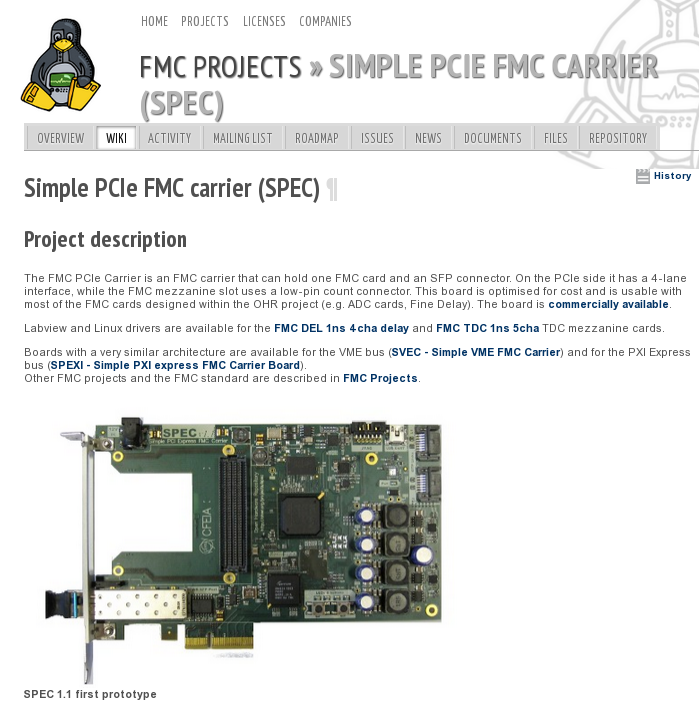
\includegraphics[scale=1]{img-poster/WEPGF089f5}
            \end{center}
                 \begin{center}
                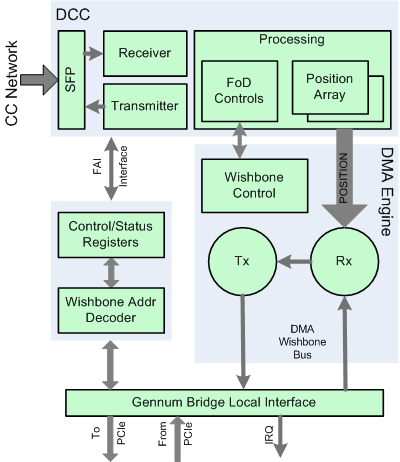
\includegraphics[scale=1.1]{img/WEPGF089f6}
                \end{center}
                By studying the open-source schematics and reference firmware design available on the repository, we were able to identify the modifications to be taken towards implementing the FA Archiver on the SPEC card.
                \begin{itemize}
                    \setlength\itemsep{1em}
                    \item PCIe Interface uses on-board Gennum PCIe bridge.
                    \item Clocking Resources uses on-board programmable oscillator for Communication Controller.
                    \item SoC Communication uses Wishbone bus.
                \end{itemize}
            \end{multicols*}
        }
\end{columns}

\end{document}
